\chapter{Periodicidade}\label{ch:b1:periodicity}

Lítio, sódio e potássio são metais moles e brilhantes que escurecem ao
ar e reagem com a água; flúor, cloro e bromo são não metais coloridos e
corrosivos, que arrancam elétrons de quase tudo. Cada trio ocupa uma
coluna da tabela periódica, e os membros de uma coluna se parecem entre
si, enquanto os vizinhos ao longo de uma linha não. O capítulo anterior
explicou por quê: os elementos de uma coluna têm a mesma configuração
dos \omterm{def:b1:quantum-numbers:configuration}{elétrons de valência}. Este capítulo transforma essa explicação em
números --- raios, energias de ionização, \omterm{def:b1:periodicity:electron-affinity}{afinidades eletrônicas},
\omterm{def:b1:periodicity:electronegativity}{eletronegatividades} --- e nas tendências que permitem ao químico prever,
apenas pela posição de um elemento, o tamanho de seus átomos, a
facilidade com que cedem ou aceitam elétrons e para que lado se inclinam
os elétrons de uma ligação.

\begin{recall}
Todo \omterm{def:b1:periodicity:table}{período} começa com o preenchimento de uma \omterm{def:b1:quantum-numbers:orbital}{subcamada} $n$s e termina
com uma \omterm{def:b1:quantum-numbers:orbital}{subcamada} $n$p completa; os \omterm{def:b1:periodicity:table}{blocos} s, p, d e f têm larguras 2, 6,
10 e 14 (\cref{prop:b1:quantum-numbers:table}). O Livro 1 (ano 11)
descreveu a \omterm{def:b1:periodicity:electronegativity}{eletronegatividade} como a tendência de um átomo a atrair os
elétrons de uma ligação.
\end{recall}

\section{A tabela construída a partir das configurações}

\begin{definition}[Período, grupo, bloco]\label{def:b1:periodicity:table}
Na tabela periódica, os elementos são dispostos em ordem crescente de
número atômico $Z$. Um \emph{período}\index{periodo@período} é uma linha:
os elementos cuja camada de valência tem o mesmo número principal $n$.
Um \emph{grupo}\index{grupo} é uma coluna, numerada de 1 a 18: os
elementos com a mesma configuração de valência. Um \emph{bloco}\index{bloco} é o
conjunto dos elementos cuja última \omterm{def:b1:quantum-numbers:orbital}{subcamada} preenchida é de um mesmo
tipo, s, p, d ou f.
\end{definition}

\begin{example}[Ler uma posição]\label{ex:b1:periodicity:position}
O selênio, $[\ce{Ar}]\,3\text{d}^{10} 4\text{s}^2 4\text{p}^4$, está no
\omterm{def:b1:periodicity:table}{período} 4 (camada de valência $n = 4$), no \omterm{def:b1:periodicity:table}{bloco} p e no \omterm{def:b1:periodicity:table}{grupo} 16 (dois
elétrons s, dez d e quatro p: $2 + 10 + 4$); sua configuração de valência
$n\text{s}^2 n\text{p}^4$ é a do oxigênio e do enxofre acima dele.
\end{example}

\begin{definition}[Metal, não metal, metaloide]\label{def:b1:periodicity:metalloid}
Um metal é um elemento cujo sólido conduz eletricidade e cujos átomos
perdem facilmente elétrons para formar cátions; um não metal é um
elemento que não conduz (com exceções como o grafite) e que ganha
facilmente elétrons ou os compartilha. Um \emph{metaloide}\index{metaloide} é um
elemento de caráter intermediário, um semicondutor: boro, silício,
germânio, arsênio, antimônio e telúrio.
\end{definition}

\begin{omfigure}
\omperiodictable[colour=metals, legend, f block=false]

{\small Os metais (a grande maioria), os \omterm{def:b1:periodicity:metalloid}{metaloides} ao longo de uma
escada do boro ao telúrio, e os não metais no canto superior direito. O
\omterm{def:b1:periodicity:table}{bloco} f, omitido aqui, é formado de metais.}
\end{omfigure}

\section{Tamanho: raios atômicos e iônicos}

\begin{definition}[Blindagem, carga nuclear efetiva]\label{def:b1:periodicity:screening}
Em um átomo com vários elétrons, um elétron é atraído pelo núcleo, de
carga $Ze$, e repelido pelos outros elétrons. Os elétrons internos
cancelam em parte a atração do núcleo: é a
\emph{blindagem}\index{blindagem}. O \omterm{def:b1:quantum-numbers:configuration}{elétron de valência} se comporta como se
sentisse uma carga nuclear reduzida $Z^{*}e$, a \emph{carga nuclear
efetiva}\index{carga nuclear efetiva}, com $Z^{*} < Z$. Os elétrons de
uma camada interna blindam quase completamente; os elétrons da mesma
camada blindam apenas um pouco.
\end{definition}

\begin{remark}[Uma ferramenta qualitativa]\label{rem:b1:periodicity:slater}
Neste livro, $Z^{*}$ é usada de forma qualitativa: ao longo de um
\omterm{def:b1:periodicity:table}{período}, $Z$ aumenta de uma unidade a cada passo, enquanto o elétron
acrescentado, na mesma camada, blinda apenas um pouco, de modo que a
$Z^{*}$ sentida pelos \omterm{def:b1:quantum-numbers:configuration}{elétrons de valência} aumenta; descendo um grupo,
$Z^{*}$ varia pouco, mas a camada de valência
$n$ cresce. As regras para calcular $Z^{*}$ a partir da configuração (as
regras de Slater) são dadas no volume do 2.º ano.
\end{remark}

\begin{definition}[Raio covalente, raio iônico]\label{def:b1:periodicity:radius}
O \emph{raio covalente}\index{raio covalente} de um elemento é a metade
do comprimento de uma ligação simples entre dois de seus átomos: para o
cloro, a metade da distância \ce{Cl-Cl} em \ce{Cl2}. O \emph{raio
iônico}\index{raio ionico@raio iônico} de um íon é a parcela da distância
entre cátions e ânions vizinhos nos cristais iônicos que lhe é
atribuída, segundo uma convenção que fixa o raio de um íon de referência
(\ce{O^{2-}}); ele depende ligeiramente do número de vizinhos.
\end{definition}

\begin{example}[Os halogênios]\label{ex:b1:periodicity:halogen-radii}
Os comprimentos de ligação de \ce{F2}, \ce{Cl2}, \ce{Br2} e \ce{I2} são 141.2,
198.8, 228.1 e \qty{266.6}{pm}, de modo que os \omterm{def:b1:periodicity:radius}{raios covalentes} são 71, 99, 114
e \qty{133}{pm}: cada passo para baixo no grupo acrescenta uma camada e cerca de
\qty{20}{pm} ou mais.
% ledger: re:F2, re:Cl2, re:Br2, re:I2
\end{example}

\begin{proposition}[Tendências do raio]\label{prop:b1:periodicity:radius-trend}
Os raios atômicos diminuem da esquerda para a direita ao longo de um
\omterm{def:b1:periodicity:table}{período} e aumentam de cima para baixo em um grupo. Um cátion é menor que
seu átomo, um ânion é maior; em uma série isoeletrônica (íons com a mesma
configuração), o raio diminui quando $Z$ aumenta.
\end{proposition}

\begin{proof}[Raciocínio]
O tamanho de um átomo é o tamanho de seus orbitais de valência, que se
contraem quando $Z^{*}$ cresce e se dilatam quando $n$ cresce. Ao longo
de um \omterm{def:b1:periodicity:table}{período}, $n$ é fixo e $Z^{*}$ cresce: os átomos se contraem.
Descendo um grupo, $n$ aumenta de uma unidade a cada passo, o que supera
a pequena variação de $Z^{*}$. Um cátion perdeu sua camada de valência,
ou elétrons que se repeliam; um ânion ganhou um elétron que repele os
outros. Em uma série isoeletrônica, os mesmos elétrons são retidos por
um núcleo de carga crescente.
\end{proof}

\begin{omfigure}
\begin{tikzpicture}[font=\small, x=1pt, y=1pt]
  % ledger: rion:O2-VI, rion:F-VI, rion:Na+VI, rion:Mg2+VI, rion:Al3+VI
  % radii in pm drawn at 0.30 pt per pm (circles to scale)
  \foreach \x/\r/\lab/\v in {40/140/\ce{O^{2-}}/140, 130/133/\ce{F-}/133,
      210/102/\ce{Na+}/102, 275/72/\ce{Mg^{2+}}/72, 325/53.5/\ce{Al^{3+}}/54} {
    \draw[fill=omDef!20, draw=omDef!70!black] (\x,0) circle ({0.30*\r});
    \node at (\x,0) {\lab};
    \node[below] at (\x,-50) {\v\,pm};
  }
  \node[anchor=west, align=left] at (350,0) {dez elétrons cada,\\$Z = 8 \to 13$};
\end{tikzpicture}

{\small A série isoeletrônica $1\text{s}^2 2\text{s}^2 2\text{p}^6$,
desenhada em escala (\omterm{def:b1:periodicity:radius}{raios iônicos} para seis vizinhos). Os mesmos dez
elétrons se contraem à medida que a carga nuclear cresce.}
\end{omfigure}

\section{Energias: ionização e afinidade eletrônica}

\begin{definition}[Energias de ionização]\label{def:b1:periodicity:ionisation-energy}
A \emph{primeira energia de ionização}\index{primeira energia de ionizacao@primeira energia de ionização} $E_{i1}$
de um elemento é a energia necessária para retirar um elétron do átomo
isolado em seu \omterm{def:b1:quantum-numbers:energy-level}{estado fundamental}, em fase gasosa:
\[
  \ce{X(g) -> X+(g) + e-}, \qquad E_{i1} = E(\ce{X+}) + E(\ce{e-}) - E(\ce{X}) > 0 .
\]
As \emph{energias de ionização sucessivas}\index{energias de ionizacao sucessivas@energias de ionização sucessivas}
$E_{i2}, E_{i3}, \dots$ retiram o segundo, o terceiro
elétron\dots\ de \ce{X+}, \ce{X^{2+}}\dots\ Elas são expressas em
elétron-volts por átomo ou em quilojoules por mol
($\qty{1}{eV} \leftrightarrow \qty{96.49}{kJ/mol}$).
% ledger: const:NA, const:e (1 eV x N_A = 96.485 kJ/mol)
\end{definition}

\begin{omfigure}
\begin{tikzpicture}
\begin{axis}[
  width=0.92\linewidth, height=6.4cm,
  xmin=0, xmax=37, ymin=0, ymax=27,
  axis x line=bottom, axis y line=left,
  xlabel={número atômico $Z$}, ylabel={$E_{i1}$ (eV)},
  xtick={2,10,18,36}, ytick={0,5,10,15,20,25},
  tick label style={font=\small}, label style={font=\small},
  clip=false]
\addplot[omDef, thick, mark=*, mark size=1.3pt] table[x=Z, y=IE_eV] {figdata/out/bachelor-1-ionisation-energies.dat};
\node[font=\small, anchor=south] at (axis cs:2,24.6) {He};
\node[font=\small, anchor=south] at (axis cs:10,21.6) {Ne};
\node[font=\small, anchor=south] at (axis cs:18,15.8) {Ar};
\node[font=\small, anchor=south] at (axis cs:36,14.0) {Kr};
\node[font=\small, anchor=north] at (axis cs:3,5.2) {Li};
\node[font=\small, anchor=north] at (axis cs:11,4.9) {Na};
\node[font=\small, anchor=north] at (axis cs:19,4.1) {K};
\node[font=\small, anchor=north] at (axis cs:31,5.8) {Ga};
\node[font=\small, anchor=north] at (axis cs:5,7.9) {B};
\node[font=\small, anchor=north] at (axis cs:8,13.2) {O};
\node[font=\small, anchor=north west] at (axis cs:13.1,6.0) {Al};
\node[font=\small, anchor=north] at (axis cs:16,9.9) {S};
\node[font=\small, anchor=south] at (axis cs:26,8.0) {metais 3d};
\end{axis}
\end{tikzpicture}

{\small \omterm{def:b1:periodicity:ionisation-energy}{Primeiras energias de ionização} dos 36 primeiros elementos.
Máximos nos gases nobres, mínimos nos metais alcalinos; as pequenas
quedas em B, Al, Ga e em O, S são os efeitos de \omterm{def:b1:quantum-numbers:orbital}{subcamada} da
\cref{prop:b1:periodicity:ie-anomalies}.}
\end{omfigure}

\begin{proposition}[Tendências da energia de ionização]\label{prop:b1:periodicity:ie-trend}
A \omterm{def:b1:periodicity:ionisation-energy}{primeira energia de ionização} aumenta ao longo de um \omterm{def:b1:periodicity:table}{período}, do metal
alcalino ao gás nobre, e diminui descendo um grupo. As \omterm{def:b1:periodicity:ionisation-energy}{energias de
ionização sucessivas} sempre aumentam, $E_{i1} < E_{i2} < \dots$, e dão um
salto por um fator grande quando o elétron retirado pertence a uma camada
interna.
\end{proposition}

\begin{proof}[Raciocínio]
Retirar um elétron é mais fácil quando ele está longe do núcleo e sente
uma $Z^{*}$ pequena: ao longo de um \omterm{def:b1:periodicity:table}{período}, $Z^{*}$ cresce e o raio
diminui; descendo um grupo, o raio cresce. Cada elétron sucessivo é
arrancado de um íon de carga maior e tamanho menor, e por isso custa
mais; uma vez vazia a camada de valência, o elétron seguinte vem de uma
camada de $n$ menor, muito mais próxima do núcleo e quase sem \omterm{def:b1:periodicity:screening}{blindagem}.
\end{proof}

\begin{example}[O magnésio]\label{ex:b1:periodicity:magnesium}
As \omterm{def:b1:periodicity:ionisation-energy}{energias de ionização sucessivas} do magnésio são 7.65, 15.04, 80.14
e \qty{109.27}{eV}. A razão $E_{i2}/E_{i1} \approx 2$ é moderada;
$E_{i3}/E_{i2} \approx 5.3$ é um salto: o terceiro elétron vem do cerne
2p. O magnésio cede seus dois elétrons 3s e para em
\ce{Mg^{2+}}, que tem a configuração de gás nobre do neônio.
% ledger: ie:Mg, ie2:Mg, ie3:Mg, ie4:Mg
\end{example}

\begin{omfigure}
\begin{tikzpicture}
\begin{axis}[
  width=0.55\linewidth, height=5.2cm, ybar, bar width=14pt,
  xmin=0.4, xmax=4.6, ymin=1, ymax=300, ymode=log,
  axis x line=bottom, axis y line=left,
  xlabel={elétron retirado}, ylabel={$E_{i}$ (eV)},
  xtick={1,2,3,4}, xticklabels={1.º,2.º,3.º,4.º},
  tick label style={font=\small}, label style={font=\small},
  nodes near coords={\pgfmathprintnumber[fixed, fixed zerofill, precision=2]{\pgfplotspointmeta}},
  nodes near coords style={font=\scriptsize},
  point meta=rawy]
\addplot[fill=omDef!40, draw=omDef] table[x=k, y=IE_eV] {figdata/out/bachelor-1-ionisation-energies-mg.dat};
\end{axis}
\end{tikzpicture}

{\small \omterm{def:b1:periodicity:ionisation-energy}{Energias de ionização sucessivas} do magnésio (eixo logarítmico).
A terceira vale cinco vezes a segunda: a camada 3s está vazia e o cerne
é alcançado.}
\end{omfigure}

\begin{proposition}[Duas quedas ao longo de um período]\label{prop:b1:periodicity:ie-anomalies}
Ao longo dos \omterm{def:b1:periodicity:table}{períodos} 2 e 3, a \omterm{def:b1:periodicity:ionisation-energy}{primeira energia de ionização} cai
ligeiramente do \omterm{def:b1:periodicity:table}{grupo} 2 para o \omterm{def:b1:periodicity:table}{grupo} 13 (\ce{Be} para \ce{B}, \ce{Mg}
para \ce{Al}) e do \omterm{def:b1:periodicity:table}{grupo} 15 para o \omterm{def:b1:periodicity:table}{grupo} 16 (\ce{N} para \ce{O}, \ce{P}
para \ce{S}).
\end{proposition}

\begin{proof}[Raciocínio]
Em \ce{B} e \ce{Al}, o elétron retirado é o primeiro elétron p, mais
alto em energia que os elétrons s de \ce{Be} e \ce{Mg}. Em \ce{O}
e \ce{S}, o elétron retirado é o quarto elétron p, o primeiro a
compartilhar um orbital (\omorbs{ud,u,u}): sua repulsão com o parceiro
torna mais fácil retirá-lo do que um elétron da \omterm{def:b1:quantum-numbers:orbital}{subcamada} semipreenchida
de \ce{N} ou \ce{P} (\omorbs{u,u,u}).
% ledger: ie:Be, ie:B, ie:N, ie:O, ie:Mg, ie:Al, ie:P, ie:S
\end{proof}

\begin{definition}[Afinidade eletrônica]\label{def:b1:periodicity:electron-affinity}
A \emph{afinidade eletrônica}\index{afinidade eletronica@afinidade eletrônica} $E_{ea}$ de um
elemento é a energia liberada quando um átomo isolado em seu \omterm{def:b1:quantum-numbers:energy-level}{estado
fundamental} captura um elétron em fase gasosa,
\[
  \ce{X(g) + e- -> X-(g)}, \qquad E_{ea} = E(\ce{X}) + E(\ce{e-}) - E(\ce{X-}) .
\]
Ela é positiva quando o ânion é mais estável que o átomo e o elétron
livre.
\end{definition}

\begin{example}[Os halogênios e seus vizinhos]\label{ex:b1:periodicity:ea}
As \omterm{def:b1:periodicity:electron-affinity}{afinidades eletrônicas} de \ce{F}, \ce{Cl}, \ce{Br} e \ce{I} são 3.40,
3.61, 3.36 e \qty{3.06}{eV}, as maiores de todos os elementos; as de
\ce{O} e \ce{S} são 1.44 e \qty{2.02}{eV}, a de \ce{C} \qty{1.26}{eV},
a de \ce{Na} \qty{0.55}{eV}. Os átomos que completam uma \omterm{def:b1:quantum-numbers:orbital}{subcamada} ao
capturar um elétron (os halogênios) liberam muita energia. Nitrogênio,
berílio, magnésio e os gases nobres não formam ânion gasoso estável: o
elétron extra teria de se emparelhar em uma \omterm{def:b1:quantum-numbers:orbital}{subcamada} p semipreenchida
ou entrar em uma nova \omterm{def:b1:quantum-numbers:orbital}{subcamada}. A afinidade do flúor é menor que a do
cloro porque o elétron acrescentado fica comprimido na pequena camada 2p.
% ledger: ea:F, ea:Cl, ea:Br, ea:I, ea:O, ea:S, ea:C, ea:Na
\end{example}

\section{Eletronegatividade e polarizabilidade}

\begin{definition}[Eletronegatividade]\label{def:b1:periodicity:electronegativity}
A \emph{eletronegatividade}\index{eletronegatividade} $\chi$ de um
elemento mede a tendência de seus átomos, em uma molécula, a atrair
os elétrons das ligações que formam. Duas escalas são usadas.
\begin{itemize}
  \item Na \emph{escala de Pauling}\index{escala de Pauling}, as diferenças
        são definidas a partir das energias de ligação $D$:
        \[
          |\chi_A - \chi_B| = \sqrt{\frac{\Delta E}{\qty{1}{eV}}}, \qquad
          \Delta E = D(\text{A--B}) - \tfrac12\big[D(\text{A--A}) +
          D(\text{B--B})\big],
        \]
        e a escala é ancorada por $\chi(\ce{F}) = 3.98$.
  \item Na \emph{escala de Mulliken}\index{escala de Mulliken},
        $\chi_M = \tfrac12\,(E_{i1} + E_{ea})$, em elétron-volts.
\end{itemize}
\end{definition}

\begin{remark}[Por que a energia de ligação extra]\label{rem:b1:periodicity:pauling}
Se os dois átomos de uma ligação A--B atraíssem igualmente seus
elétrons, a energia da ligação seria aproximadamente a média das de A--A
e B--B. Quando um átomo é mais eletronegativo, a ligação adquire um
caráter iônico parcial, $\ce{A^{\delta+}-B^{\delta-}}$, cuja atração
eletrostática acrescenta energia: $\Delta E > 0$ mede o compartilhamento
desigual. A definição de Mulliken diz o mesmo do ponto de vista dos
átomos: um átomo que retém fortemente os próprios elétrons ($E_i$
grande) e acolhe bem um elétron extra
($E_{ea}$ grande) atrai os elétrons de uma ligação.
\end{remark}

\begin{omfigure}
% ledger: en:H, en:Li, en:Be, en:B, en:C, en:N, en:O, en:F, en:Na, en:Mg,
% en:Al, en:Si, en:P, en:S, en:Cl, en:K, en:Ca, en:Ga, en:Ge, en:As, en:Se,
% en:Br, en:Rb, en:Sr, en:In, en:Sn, en:Sb, en:Te, en:I, en:Cs, en:Ba
\omperiodictable[upto=56, f block=false, numbers=false, highlight colour=omDef!12,
  highlight={F,O,N,Cl}, values={H/2.20,Li/0.98,Be/1.57,B/2.04,C/2.55,N/3.04,O/3.44,F/3.98,
  Na/0.93,Mg/1.31,Al/1.61,Si/1.90,P/2.19,S/2.58,Cl/3.16,K/0.82,Ca/1.00,Ga/1.81,Ge/2.01,
  As/2.18,Se/2.55,Br/2.96,Rb/0.82,Sr/0.95,In/1.78,Sn/1.96,Sb/2.05,Te/2.10,I/2.66,
  Cs/0.79,Ba/0.89}]

{\small \omterm{def:b1:periodicity:electronegativity}{Eletronegatividades} de Pauling dos elementos representativos (o
\omterm{def:b1:periodicity:table}{bloco} d foi deixado em branco). Elas aumentam da esquerda para a direita
e de baixo para cima; os quatro elementos mais eletronegativos, F, O, Cl
e N, estão sombreados.}
\end{omfigure}

\begin{proposition}[Tendências da eletronegatividade]\label{prop:b1:periodicity:en-trend}
A \omterm{def:b1:periodicity:electronegativity}{eletronegatividade} aumenta ao longo de um \omterm{def:b1:periodicity:table}{período} e diminui descendo
um grupo: o flúor é o elemento mais eletronegativo, o césio e o frâncio
os menos eletronegativos. A diferença $\Delta\chi$ entre dois átomos
ligados indica o caráter da ligação: $\Delta\chi < 0.4$ covalente quase
apolar, $0.4 < \Delta\chi < 1.7$ covalente polar, $\Delta\chi > 1.7$
predominantemente iônica --- três regiões de um contínuo, e não classes
bem delimitadas.
\end{proposition}

\begin{example}[Três ligações]\label{ex:b1:periodicity:bonds}
\ce{C-H}: $\Delta\chi = 2.55 - 2.20 = 0.35$, quase apolar;
\ce{O-H}: $3.44 - 2.20 = 1.24$, polar, com o oxigênio portando uma carga
parcial negativa; \ce{Na-Cl}: $3.16 - 0.93 = 2.23$, iônica.
% ledger: en:C, en:H, en:O, en:Na, en:Cl
\end{example}

\begin{definition}[Polarizabilidade]\label{def:b1:periodicity:polarisability}
A \emph{polarizabilidade}\index{polarizabilidade} de um átomo, íon ou
molécula mede a facilidade com que sua nuvem eletrônica é deformada por
um campo elétrico --- o campo de um íon ou de um dipolo vizinho. Uma
espécie polarizável adquire, em um campo, um momento dipolar induzido
proporcional ao campo.
\end{definition}

\begin{proposition}[Tendências da polarizabilidade]\label{prop:b1:periodicity:polarisability-trend}
A \omterm{def:b1:periodicity:polarisability}{polarizabilidade} cresce com o tamanho da nuvem eletrônica e com o
número de elétrons, e diminui com a carga do núcleo que os retém: ela
aumenta descendo um grupo ($\ce{F-} < \ce{Cl-} < \ce{Br-} <
\ce{I-}$), os ânions são muito mais polarizáveis que os cátions, e
ânions grandes e moles como \ce{I-} são as espécies comuns mais
polarizáveis.
\end{proposition}

\begin{example}[Por que a polarizabilidade importa]\label{ex:b1:periodicity:pol}
A atração de London entre moléculas, assunto do
\cref{ch:b1:intermolecular-forces-solvents}, cresce com a \omterm{def:b1:periodicity:polarisability}{polarizabilidade}:
o di-iodo é sólido à temperatura ambiente, o dicloro é um gás. Em um
cristal iônico, um cátion pequeno e muito carregado polariza um ânion
grande e confere à ligação certo caráter covalente, a falha do modelo
iônico simples encontrada no \cref{ch:b1:crystals-ionic-covalent}.
\end{example}

\begin{history}[A escala de Pauling, 1932]
Em 1932, o químico norte-americano Linus Pauling notou que a energia de
uma ligação entre dois átomos diferentes é quase sempre maior que a
média das energias das duas ligações simétricas, e construiu a partir
desse excesso a primeira escala de \omterm{def:b1:periodicity:electronegativity}{eletronegatividade}. Revista à medida
que se mediam melhores energias de ligação, sua escala ainda é a de todas
as tabelas. Pauling recebeu o Prêmio Nobel de Química em 1954, por seu
trabalho sobre a ligação química, e o Prêmio Nobel da Paz em 1962.
\end{history}

\begin{omfigure}
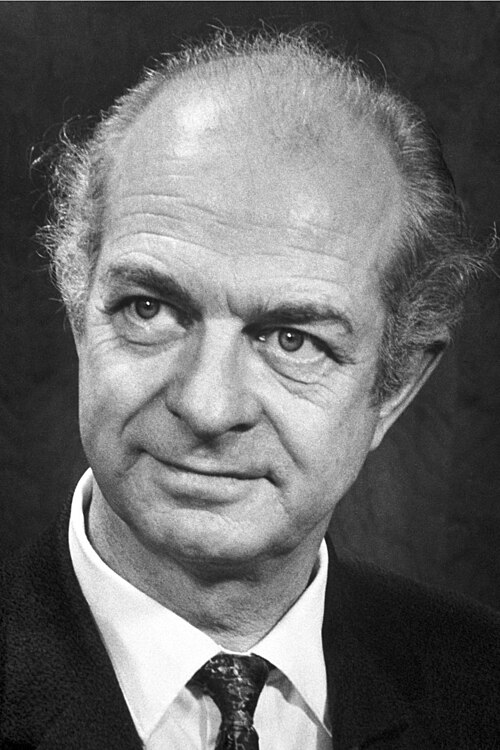
\includegraphics[width=0.24\linewidth]{images/book2/pauling.jpg}

{\small Linus Pauling (1901--1994).}
\end{omfigure}

\section{Tendências do caráter químico}

\begin{proposition}[Caráter redutor e oxidante]\label{prop:b1:periodicity:redox-trend}
Os elementos de baixa energia de ionização e baixa \omterm{def:b1:periodicity:electronegativity}{eletronegatividade}, à
esquerda da tabela e na parte de baixo de seus grupos, perdem elétrons
facilmente: são metais redutores (sobretudo os metais alcalinos). Os
elementos de alta \omterm{def:b1:periodicity:electronegativity}{eletronegatividade} e alta \omterm{def:b1:periodicity:electron-affinity}{afinidade eletrônica}, no
canto superior direito, ganham elétrons facilmente: são não metais
oxidantes (sobretudo flúor, oxigênio e cloro). Os gases nobres, com alta
energia de ionização e nenhuma afinidade por um elétron extra, não fazem
nem uma coisa nem outra.
\end{proposition}

\begin{method}[Prever uma tendência a partir da posição]\label{met:b1:periodicity:predict}
Para comparar dois elementos quanto a uma propriedade ligada à força com
que o núcleo retém os \omterm{def:b1:quantum-numbers:configuration}{elétrons de valência} (raio, $E_i$, $E_{ea}$, $\chi$):
\begin{enumerate}
  \item se estão no mesmo grupo, o de baixo tem o maior
        $n$: raio maior, $E_i$ e $\chi$ menores;
  \item se estão no mesmo \omterm{def:b1:periodicity:table}{período}, o mais à direita tem a
        maior $Z^{*}$: raio menor, $E_i$ e $\chi$ maiores;
  \item caso contrário, compare cada um com o elemento no cruzamento de
        sua linha com a coluna do outro;
  \item verifique os efeitos de \omterm{def:b1:quantum-numbers:orbital}{subcamada} (início de uma \omterm{def:b1:quantum-numbers:orbital}{subcamada} p,
        primeiro elétron p emparelhado) antes de concluir sobre as
        energias de ionização.
\end{enumerate}
\end{method}

\begin{example}[O lítio em uma bateria]\label{ex:b1:periodicity:lithium}
O lítio tem a menor \omterm{def:b1:periodicity:electronegativity}{eletronegatividade} do \omterm{def:b1:periodicity:table}{período} 2 e perde facilmente
seu elétron 2s, além de ser o metal mais leve: ele transporta mais carga
transferível por grama que qualquer outro elemento, razão pela qual
alimenta as baterias recarregáveis. Sua \omterm{def:b1:periodicity:ionisation-energy}{primeira energia de ionização},
\qty{5.39}{eV}, é maior que a do sódio (5.14) ou do potássio (4.34), e no
entanto em água ele é o metal alcalino mais redutor, paradoxo resolvido
pela forte hidratação do pequeno íon \ce{Li+} (\cref{ch:b1:nernst}).
% ledger: ie:Li, ie:Na, ie:K
\end{example}

\section{Exercícios}

\begin{exercise}[$\star$]\label{exo:b1:periodicity:1}
Dê o \omterm{def:b1:periodicity:table}{período}, o grupo e o \omterm{def:b1:periodicity:table}{bloco} do cálcio, do ferro, do selênio e do
iodo ($Z = 20, 26, 34, 53$), a partir de suas configurações.
\end{exercise}

\begin{exercise}[$\star$]\label{exo:b1:periodicity:2}
Em cada par, qual espécie é maior, e por quê? \ce{Na} ou \ce{Cl};
\ce{Na} ou \ce{Na+}; \ce{F-} ou \ce{Cl-}; \ce{Na+} ou \ce{Mg^{2+}}.
\end{exercise}

\begin{exercise}[$\star$]\label{exo:b1:periodicity:3}
As \omterm{def:b1:periodicity:ionisation-energy}{primeiras energias de ionização} de \ce{Na}, \ce{Mg}, \ce{Al}, \ce{P},
\ce{S} e \ce{Ar} são 5.14, 7.65, 5.99, 10.49, 10.36 e
\qty{15.76}{eV}. Ordene-as e aponte os dois desvios em relação à
tendência geral.
\end{exercise}

\begin{exercise}[$\star$]\label{exo:b1:periodicity:4}
Defina a \omterm{def:b1:periodicity:polarisability}{polarizabilidade} de uma espécie. Qual é mais polarizável, \ce{F-}
ou \ce{I-}? \ce{Na+} ou \ce{Cl-}? Justifique.
\end{exercise}

\begin{exercise}[$\star\star$]\label{exo:b1:periodicity:5}
As quatro \omterm{def:b1:periodicity:ionisation-energy}{primeiras energias de ionização} de um elemento do \omterm{def:b1:periodicity:table}{período} 3 são
5.99, 18.83, 28.45 e \qty{119.99}{eV}. Calcule as razões sucessivas e
identifique o elemento e o íon que ele forma.
\end{exercise}

\begin{exercise}[$\star\star$]\label{exo:b1:periodicity:6}
Explique por que o cloro tem \omterm{def:b1:periodicity:electron-affinity}{afinidade eletrônica} maior que a do flúor,
e por que o nitrogênio e o magnésio não formam ânion gasoso estável.
\end{exercise}

\begin{exercise}[$\star\star$]\label{exo:b1:periodicity:7}
Calcule as \omterm{def:b1:periodicity:electronegativity}{eletronegatividades} de Mulliken do sódio ($E_{i1} =
\qty{5.14}{eV}$, $E_{ea} = \qty{0.55}{eV}$) e do cloro ($E_{i1} =
\qty{12.97}{eV}$, $E_{ea} = \qty{3.61}{eV}$). O que elas dizem sobre a
ligação em \ce{NaCl}?
\end{exercise}

\begin{exercise}[$\star\star$]\label{exo:b1:periodicity:8}
Com os valores de Pauling do \cref{ex:b1:periodicity:bonds} e $\chi(\ce{F})
= 3.98$, classifique as ligações \ce{H-F}, \ce{C-H}, \ce{Na-Cl}, \ce{C-Cl}
($\chi(\ce{Cl}) = 3.16$) e \ce{O-H}, e dê o sinal da carga parcial
de cada átomo.
\end{exercise}

\begin{exercise}[$\star\star$]\label{exo:b1:periodicity:9}
As \omterm{def:b1:periodicity:ionisation-energy}{primeiras energias de ionização} de \ce{Li}, \ce{Na} e \ce{K} são 5.39,
5.14 e \qty{4.34}{eV}. Explique a tendência e preveja se a do
rubídio está acima ou abaixo de \qty{4.34}{eV}.
\end{exercise}

\begin{exercise}[$\star\star\star$]\label{exo:b1:periodicity:10}
O zinco ($Z = 30$) tem \omterm{def:b1:periodicity:ionisation-energy}{primeira energia de ionização} de \qty{9.39}{eV} e
o gálio ($Z = 31$), de \qty{6.00}{eV}; o arsênio ($Z = 33$), \qty{9.79}{eV},
e o selênio ($Z = 34$), \qty{9.75}{eV}. Explique as duas quedas usando as
configurações.
\end{exercise}

\begin{exercise}[$\star\star\star$]\label{exo:b1:periodicity:11}
Considere $D(\ce{H-H}) = \qty{436}{kJ/mol}$, $D(\ce{F-F}) =
\qty{158}{kJ/mol}$, $\chi(\ce{H}) = 2.20$ e $\chi(\ce{F}) = 3.98$, com
$\qty{1}{eV} = \qty{96.5}{kJ/mol}$. Use a definição de Pauling para estimar
a energia de ligação $D(\ce{H-F})$. Por que ela é tão maior que a média
das duas ligações simétricas?
\end{exercise}

\begin{exercise}[$\star\star\star$]\label{exo:b1:periodicity:12}
As \omterm{def:b1:periodicity:electronegativity}{eletronegatividades} de Pauling são tabeladas para o criptônio (3.00) e
o xenônio (2.60), mas não para o hélio, o neônio ou o argônio. Usando a
definição da escala, explique por que só se pode dar um valor para um
elemento que forma ligações, e por que são os gases nobres mais pesados
que as formam.
% ledger: en:Kr, en:Xe
\end{exercise}

\section{Problema: A aritmética de Pauling}

\begin{problem}[{Problema de fim de semana --- um elemento desconhecido a
partir de suas energias de ionização, uma série de íons com nuvens do
mesmo tamanho, duas escalas de eletronegatividade e o número de Pauling
para a ligação H--Cl}]
\label{pb:b1:periodicity:1}
Dado: $\qty{1}{eV}$ por partícula corresponde a \qty{96.485}{kJ/mol}.

\medskip
\noindent\textbf{Parte I --- Um elemento desconhecido.}
As quatro \omterm{def:b1:periodicity:ionisation-energy}{primeiras energias de ionização} de um elemento X do \omterm{def:b1:periodicity:table}{período} 3
são 7.65, 15.04, 80.14 e \qty{109.27}{eV}.
\begin{enumerate}
  \item Por que cada energia de ionização é maior que a anterior?
  \item Calcule as razões $E_{i2}/E_{i1}$, $E_{i3}/E_{i2}$ e
        $E_{i4}/E_{i3}$.
  \item Deduza o grupo de X e, em seguida, identifique-o.
  \item Que íon X forma em seus compostos? Dê sua configuração.
  \item X é um metal ou um não metal? Justifique pela sua posição.
  \item Por que o terceiro elétron custa tanto mais que o segundo?
\end{enumerate}

\medskip
\noindent\textbf{Parte II --- Dez elétrons.}
Os \omterm{def:b1:periodicity:radius}{raios iônicos} (seis vizinhos) de \ce{O^{2-}}, \ce{F-}, \ce{Na+},
\ce{Mg^{2+}} e \ce{Al^{3+}} são 140, 133, 102, 72 e \qty{54}{pm}.
\begin{enumerate}[resume]
  \item Mostre que esses íons têm a mesma configuração.
  \item Explique a ordem dos raios.
  \item Qual dos cinco íons é o mais polarizável, e por quê?
  \item Calcule a razão entre o maior e o menor raio.
  \item O comprimento de ligação de \ce{Cl2} é \qty{198.8}{pm} e o raio de
        \ce{Cl-}, \qty{181}{pm}. Calcule o \omterm{def:b1:periodicity:radius}{raio covalente} do cloro
        e compare.
  \item Sem outros dados, ordene \ce{Cl-}, \ce{Na+} e \ce{Mg^{2+}}
        por tamanho.
\end{enumerate}

\medskip
\noindent\textbf{Parte III --- A \omterm{def:b1:periodicity:electronegativity}{escala de Mulliken}.}
\begin{center}
\small
\begin{tabular}{lccccc}
\hline
elemento & \ce{F} & \ce{Cl} & \ce{Br} & \ce{O} & \ce{C} \\
\hline
$E_{i1}$ (eV) & 17.42 & 12.97 & 11.81 & 13.62 & 11.26 \\
$E_{ea}$ (eV) & 3.40 & 3.61 & 3.36 & 1.44 & 1.26 \\
$\chi$ de Pauling & 3.98 & 3.16 & 2.96 & 3.44 & 2.55 \\
\hline
\end{tabular}
\end{center}
% ledger: ie:F, ie:Cl, ie:Br, ie:O, ie:C, ea:F, ea:Cl, ea:Br, ea:O, ea:C,
% en:F, en:Cl, en:Br, en:O, en:C
\begin{enumerate}[resume]
  \item Calcule as \omterm{def:b1:periodicity:electronegativity}{eletronegatividades} de Mulliken dos cinco elementos.
  \item Ordene-as em cada escala. Qual elemento fica em posição diferente?
  \item Calcule a razão $\chi_{\text{Pauling}}/\chi_M$ para os três
        halogênios. O que você observa?
  \item Sugira por que o oxigênio foge à regra dos halogênios (observe
        sua \omterm{def:b1:periodicity:electron-affinity}{afinidade eletrônica}).
  \item Qual átomo porta a carga parcial negativa em \ce{HCl}? E em
        \ce{ClF}?
  \item Com os valores tabelados ($\chi(\ce{H}) = 2.20$), a ligação \ce{H-Cl}
        é apolar, covalente polar ou iônica?
\end{enumerate}

\medskip
\noindent\textbf{Parte IV --- O número de Pauling para H--Cl.}
As entalpias padrão de formação de \ce{H(g)}, \ce{Cl(g)} e
\ce{HCl(g)} a \qty{298}{K} são 218.0, 121.3 e \qty{-92.3}{kJ/mol};
as de \ce{H2(g)} e \ce{Cl2(g)} são nulas. A energia de ligação de uma
molécula é tomada como a entalpia de sua dissociação em átomos.
% ledger: janaf:H, janaf:Cl, janaf:HCl
\begin{enumerate}[resume]
  \item Calcule $D(\ce{H-H})$ a partir de \ce{H2(g) -> 2H(g)}.
  \item Calcule $D(\ce{Cl-Cl})$.
  \item Calcule $D(\ce{H-Cl})$ a partir de \ce{HCl(g) -> H(g) + Cl(g)}.
  \item Calcule o excesso de energia de Pauling $\Delta E$ em kJ/mol e mostre
        que ele é igual a $-\Delta_f H(\ce{HCl})$.
  \item Converta $\Delta E$ em elétron-volts.
  \item Calcule $|\chi(\ce{Cl}) - \chi(\ce{H})|$ e compare com a
        diferença dos valores tabelados, $3.16 - 2.20$.
\end{enumerate}
\end{problem}
